\documentclass[aspectratio=169, 10pt]{beamer}

% --- Theme & Colors ---
\usetheme{Madrid}
\usecolortheme{beaver} 
\setbeamertemplate{navigation symbols}{}
\setbeamertemplate{caption}[numbered]

% --- Packages ---
\usepackage{graphicx}
\usepackage{booktabs}
\usepackage{amsmath}
\usepackage{tikz}
\usetikzlibrary{shapes.geometric, arrows, positioning}
\usepackage{hyperref}

% --- Metadata ---
\title{Generating Synthetic Raman Spectra via Conditional VAEs}
\author[Andrei Iușan, Iulian Vasile]{Andrei Iușan, Iulian Vasile \texorpdfstring{\\}{ } \scriptsize{Advisors: Ion Petre, Bogdan Oancea, Alexandru Amărioarei}}
\institute[INCDSB]{National Institute of Research and Development in Biological Sciences}
\date{\today}

\begin{document}

% -----------------------------------------------------------------------------
% SLIDE 1: Title
% -----------------------------------------------------------------------------
\begin{frame}
    \titlepage
    \begin{center}
        \scriptsize{Project: Synthetic Data Augmentation for Intraoperative Spectroscopy}
    \end{center}
\end{frame}

% -----------------------------------------------------------------------------
% SECTION 1: Context
% -----------------------------------------------------------------------------
\section{The Clinical Context}

\begin{frame}{The Problem: In-Vivo Glioma Grading}
    \begin{columns}
        \begin{column}{0.6\textwidth}
            \textbf{The Clinical Need:}
            \begin{itemize}
                \item Gliomas are the most common primary brain tumors.
                \item \textbf{Grading} (LGG vs. HGG) determines surgical strategy.
                \item Current Standard: Biopsy $\to$ Pathology (days).
                \item \textbf{Goal:} Instant, intraoperative feedback.
            \end{itemize}
            
            \vspace{1em}
            \textbf{The Solution: Raman Spectroscopy}
            \begin{itemize}
                \item Inelastic light scattering measures molecular fingerprints (Lipids, Proteins, DNA).
                \item Non-destructive, label-free, instant.
            \end{itemize}
        \end{column}
        \begin{column}{0.4\textwidth}
            \begin{alertblock}{The Challenge}
                Biological heterogeneity is high, but dataset sizes are tiny ($N < 60$ patients).
            \end{alertblock}
        \end{column}
    \end{columns}
\end{frame}

\begin{frame}{The Mathematical Formulation}
    We treat each patient spectrum $x \in \mathbb{R}^{1738}$ as a sample from a high-dimensional distribution.
    \vspace{1em}
    \textbf{The Classification Task:}
    $$ f: \mathbb{R}^{1738} \to \{0, \dots, 5\} $$
    Distinguish between \textbf{6 Molecular Subtypes} (LGm1--LGm6).
    \vspace{1em}
    \begin{block}{The "Small Data" Curse}
        \begin{itemize}
            \item The "Patient Effect" dominates the signal: $Var(\text{Patient}) \gg Var(\text{Tumor})$.
            \item Standard classifiers (SVM, RF) overfit to the patient manifold, failing to generalize.
        \end{itemize}
    \end{block}
\end{frame}

% -----------------------------------------------------------------------------
% SECTION 2: The Baseline
% -----------------------------------------------------------------------------
\section{Baseline Analysis}

\begin{frame}{Establishing the Baseline (APOLLO paper)}
    To quantify the difficulty, we use the APOLLO paper's approach with a \textbf{Random Forest + SVM pipeline}.
    
    \vspace{1em}
    \textbf{Methodology:}
    \begin{itemize}
        \item \textbf{Input:} Raw Raman Spectra ($1738$ features).
        \item \textbf{Validation Scheme:} 5-Fold \textit{Patient-Wise} Cross Validation.
        \item \textbf{Constraint:} Strict splitting ensures no patient appears in both Train and Test sets.
    \end{itemize}
    
    \vspace{1em}
    \begin{alertblock}{Preliminary Observation}
        Initial experiments indicate that standard classifiers struggle to separate the fine-grained molecular subtypes when tested on unseen patients. This confirms the need for \textbf{manifold learning} and data augmentation to bridge the gap between training and testing distributions.
    \end{alertblock}
\end{frame}

% -----------------------------------------------------------------------------
% NEW SLIDE: Evaluation Methodology
% -----------------------------------------------------------------------------
\begin{frame}{Evaluation Methodology: Dual Objectives}
    Since our architecture serves two purposes, we define two distinct evaluation protocols to benchmark against the baseline.
    
    \vspace{1em}
    \begin{columns}[t]
        \column{0.5\textwidth}
        \textbf{1. Classification Objective}
        \begin{itemize}
            \item \textbf{Goal:} Improve direct diagnosis.
            \item \textbf{Mechanism:} The CVAE Encoder has an \textit{Auxiliary Classification Head}.
            \item \textbf{Metric:} Compare the validation accuracy of the \textbf{CVAE Encoder} directly against the \textbf{RF/SVM Baseline}.
            \item \textit{Hypothesis:} The regularization from the generative task might improve feature robustness.
        \end{itemize}

        \column{0.5\textwidth}
        \textbf{2. Synthesis Objective (TSTR)}
        \begin{itemize}
            \item \textbf{Goal:} Prove synthetic data utility.
            \item \textbf{Metric:} \textbf{T}rain on \textbf{S}ynthetic, \textbf{T}est on \textbf{R}eal.
            \begin{enumerate}
                \item Train CVAE on Real Data.
                \item Generate 10k Synthetic Samples.
                \item Train a \textit{fresh} classifier on Synthetic.
                \item Test on Real Patients.
            \end{enumerate}
            \item \textit{Success:} If $Acc_{TSTR} \approx Acc_{TRTR}$, the synthetic data is biologically valid.
        \end{itemize}
    \end{columns}
\end{frame}

% -----------------------------------------------------------------------------
% SECTION 3: Method (CVAE)
% -----------------------------------------------------------------------------
\section{Generative Solution}
%---------------------------------------------------------

\section{Proposed Solution}

\begin{frame}{Concept: The Variational Autoencoder (VAE)}
    \centering
    The VAE imposes a probabilistic bottleneck to learn a continuous latent manifold $\mathcal{Z}$.
    
    \vspace{1em}
    
    % TikZ Diagram for Standard VAE
    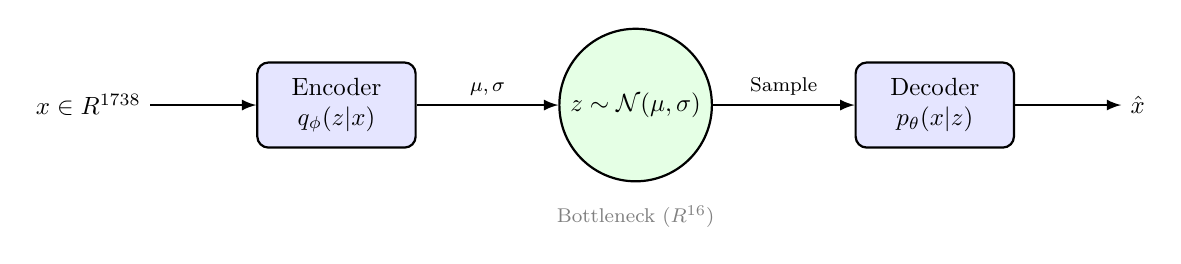
\begin{tikzpicture}[node distance=1.5cm, auto, >=latex, thick, scale=0.9, transform shape]
        % Styles
        \tikzstyle{block} = [rectangle, draw, fill=blue!10, text width=2cm, text centered, rounded corners, minimum height=1.2cm]
        \tikzstyle{circle_node} = [circle, draw, fill=green!10, text centered, minimum size=1cm]
        
        % Nodes
        \node (input) {$x \in \mathbb{R}^{1738}$};
        \node [block, right=of input] (encoder) {Encoder\\$q_\phi(z|x)$};
        \node [circle_node, right=of encoder, xshift=0.5cm] (latent) {$z \sim \mathcal{N}(\mu, \sigma)$};
        \node [block, right=of latent, xshift=0.5cm] (decoder) {Decoder\\$p_\theta(x|z)$};
        \node [right=of decoder] (output) {$\hat{x}$};
        
        % Edges
        \draw[->] (input) -- (encoder);
        \draw[->] (encoder) -- node[above, font=\footnotesize] {$\mu, \sigma$} (latent);
        \draw[->] (latent) -- node[above, font=\footnotesize] {Sample} (decoder);
        \draw[->] (decoder) -- (output);
        
        % Annotation
        \node[below=0.2cm of latent, font=\footnotesize, text=gray] {Bottleneck ($\mathbb{R}^{16}$)};
    \end{tikzpicture}
    
    \vspace{1em}
    \begin{itemize}
        \item Unlike standard Autoencoders, VAEs learn a \textbf{distribution}, not just a compression.
        \item This allows us to sample \textit{new} data points from the latent space.
    \end{itemize}
\end{frame}

\begin{frame}{Architecture I: Conditional Mechanism}
    We modify the VAE to include an \textbf{Auxiliary Classifier} and \textbf{Conditional Decoder}.
    
    \vspace{0.5em}
    \centering
    % TikZ Diagram for CVAE High Level
    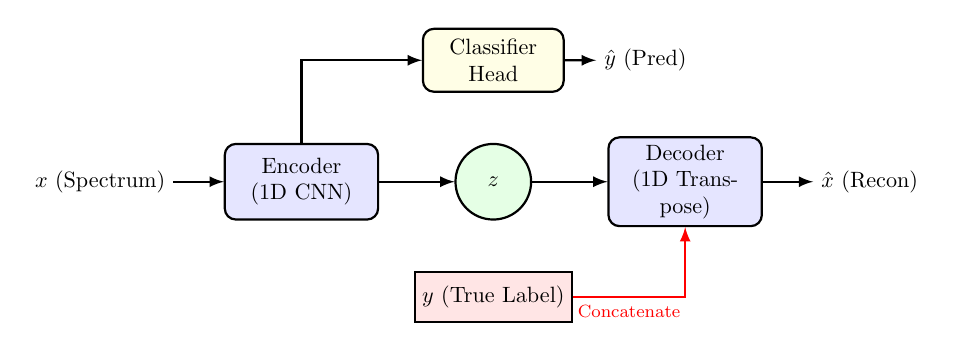
\begin{tikzpicture}[node distance=1.5cm, auto, >=latex, thick, scale=0.8, transform shape]
        % Styles
        \tikzstyle{block} = [rectangle, draw, fill=blue!10, text width=2.2cm, text centered, rounded corners, minimum height=1.2cm]
        \tikzstyle{input} = [rectangle, draw=none, fill=none]
        \tikzstyle{latent} = [circle, draw, fill=green!10, text centered, minimum size=1.2cm]
        \tikzstyle{label} = [rectangle, draw, fill=red!10, text centered, minimum height=0.8cm]
        \tikzstyle{head} = [rectangle, draw, fill=yellow!10, text width=2cm, text centered, rounded corners, minimum height=1cm]
        
        % Nodes
        \node [input] (x) {$x$ (Spectrum)};
        \node [block, right=0.8cm of x] (encoder) {Encoder\\(1D CNN)};
        \node [latent, right=1.2cm of encoder] (z) {$z$};
        \node [label, below=0.8cm of z] (y) {$y$ (True Label)};
        
        \node [block, right=1.2cm of z] (decoder) {Decoder\\(1D Transpose)};
        \node [input, right=0.8cm of decoder] (x_hat) {$\hat{x}$ (Recon)};
        
        % Aux Head (Branching off Encoder)
        \node [head, above=0.8cm of z] (classifier) {Classifier Head};
        \node [input, right=0.5cm of classifier] (y_pred) {$\hat{y}$ (Pred)};

        % Edges
        \draw[->] (x) -- (encoder);
        \draw[->] (encoder) -- (z);
        \draw[->] (encoder) |- (classifier);
        \draw[->] (classifier) -- (y_pred);
        
        % Conditioning Arrows
        \draw[->] (z) -- (decoder);
        \draw[->, color=red] (y) -| node[near start, below, font=\footnotesize, color=red] {Concatenate} (decoder);
        \draw[->] (decoder) -- (x_hat);
    \end{tikzpicture}
    
    \vspace{0.5em}
    \begin{itemize}
        \item \textbf{Disentanglement:} The Encoder learns spectral features unsupervised.
        \item \textbf{Conditioning:} Class label $y$ is injected \textbf{only} at the Decoder.
    \end{itemize}
\end{frame}

\begin{frame}{Architecture II: Asymmetric Topology}
    We propose an asymmetric design with \textbf{Skip Connections} in the Encoder to preserve multi-scale spectral features.
    
    \vspace{1em}
    \centering
    % TikZ Diagram for Asymmetric Topology
    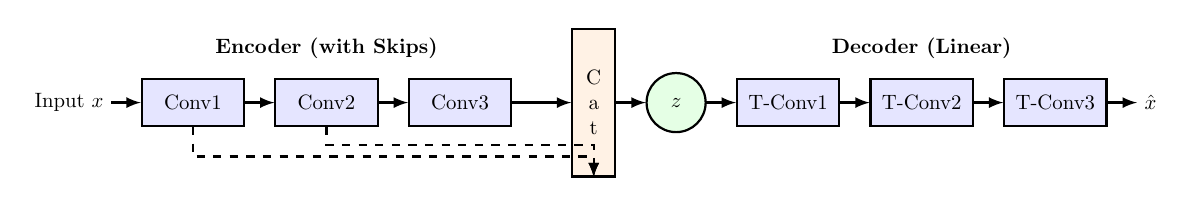
\begin{tikzpicture}[node distance=1.2cm, auto, >=latex, thick, scale=0.75, transform shape]
        % Styles
        \tikzstyle{layer} = [rectangle, draw, fill=blue!10, text width=1.5cm, text centered, minimum height=0.8cm]
        \tikzstyle{latent} = [circle, draw, fill=green!10, text centered, minimum size=1cm]
        \tikzstyle{concat} = [rectangle, draw, fill=orange!10, text centered, minimum height=2.5cm, text width=0.5cm]
        
        % ENCODER SIDE
        \node (input) {Input $x$};
        \node [layer, right=0.5cm of input] (conv1) {Conv1};
        \node [layer, right=0.5cm of conv1] (conv2) {Conv2};
        \node [layer, right=0.5cm of conv2] (conv3) {Conv3};
        
        % Concat Block
        \node [concat, right=1cm of conv3] (cat) {C\\a\\t};
        
        % Skip connections arrows
        \draw[->] (input) -- (conv1);
        \draw[->] (conv1) -- (conv2);
        \draw[->] (conv2) -- (conv3);
        
        % Skips to Concat
        \draw[->, dashed] (conv1.south) -- ++(0,-0.5) -| (cat.south);
        \draw[->, dashed] (conv2.south) -- ++(0,-0.3) -| (cat.south);
        \draw[->] (conv3) -- (cat);
        
        % Latent
        \node [latent, right=0.5cm of cat] (z) {$z$};
        \draw[->] (cat) -- (z);
        
        % DECODER SIDE (Linear/No Skips)
        \node [layer, right=0.5cm of z] (tconv1) {T-Conv1};
        \node [layer, right=0.5cm of tconv1] (tconv2) {T-Conv2};
        \node [layer, right=0.5cm of tconv2] (tconv3) {T-Conv3};
        \node [right=0.5cm of tconv3] (out) {$\hat{x}$};
        
        \draw[->] (z) -- (tconv1);
        \draw[->] (tconv1) -- (tconv2);
        \draw[->] (tconv2) -- (tconv3);
        \draw[->] (tconv3) -- (out);
        
        % Labels
        \node[above=0.2cm of conv2] {\textbf{Encoder (with Skips)}};
        \node[above=0.2cm of tconv2] {\textbf{Decoder (Linear)}};
        
    \end{tikzpicture}
    
    \vspace{1em}
    \begin{itemize}
        \item \textbf{Encoder:} $x \to \text{Conv}_1 \to \text{Conv}_2 \to \text{Conv}_3$. Output is Concat($c_1, c_2, c_3$).
        \item \textbf{Decoder:} Standard sequential Transposed Convolutions (No skips).
        \item \textbf{Rationale:} Skip connections help the encoder preserve high-frequency spectral peaks that might vanish in deep layers.
    \end{itemize}
\end{frame}

\begin{frame}{The Loss Function}
    The total objective maximizes the Evidence Lower Bound (ELBO) while minimizing classification error.
    
    $$ \mathcal{L}_{Total} = \mathcal{L}_{Recon} + \beta \mathcal{L}_{KL} + \alpha \mathcal{L}_{Class} $$
    
    \vspace{1em}
    \begin{enumerate}
        \item \textbf{Reconstruction Loss (MSE):} Ensures physical fidelity.
        $$ \mathcal{L}_{Recon} = \sum_{i=1}^{1738} || x_i - \hat{x}_i ||^2 $$
        
        \item \textbf{KL Divergence:} Regularizes latent space to be $\mathcal{N}(0, I)$.
        $$ \mathcal{L}_{KL} = -\frac{1}{2} \sum_{j=1}^{16} (1 + \log(\sigma_j^2) - \mu_j^2 - \sigma_j^2) $$
        
        \item \textbf{Classification Loss:} Cross-Entropy on the auxiliary head.
        $$ \mathcal{L}_{Class} = - \sum_{k=0}^{6} y_k \log(\hat{y}_k) $$
    \end{enumerate}
\end{frame}
% -----------------------------------------------------------------------------
% SECTION 4: Results
% -----------------------------------------------------------------------------
\section{Results}

\begin{frame}{Reconstruction Analysis}
    Does the model learn the physics? (Example from our tests with the CVAE architecture)
    \begin{figure}
        \centering
        \includegraphics[width=0.8\textwidth]{FigC_Reconstruction_Mirror.pdf}
        \caption{\textbf{Mirror Plot:} Top (Black) is Real input. Bottom (Red) is CVAE Reconstruction. Note the preservation of key spectral peaks.}
    \end{figure}
\end{frame}



% -----------------------------------------------------------------------------
% SECTION 4: Planned Evaluation
% -----------------------------------------------------------------------------
\section{Planned Evaluation}

\begin{frame}{Evaluation Strategy}
    As this is an ongoing project, we propose the following validation metrics:
    
    \vspace{1em}
    \begin{enumerate}
        \item \textbf{Manifold Quality (Visual):}
        \begin{itemize}
            \item \textbf{t-SNE Projection:} Do the 6 molecular subtypes form distinct clusters in the latent space $\mathcal{Z}$?
            \item \textbf{Generative Traversal:} Can we smoothly interpolate between subtypes (e.g., $z_{LGm1} \to z_{LGm6}$) to model the "tumor gradient"?
        \end{itemize}
        
        \vspace{1em}
        \item \textbf{Data Utility (TSTR):}
        \begin{itemize}
            \item \textbf{T}rain on \textbf{S}ynthetic, \textbf{T}est on \textbf{R}eal.
            \item We will generate 10,000 synthetic spectra and train a classifier.
            \item \textbf{Success Metric:} If Accuracy(Synthetic) $\approx$ Accuracy(Baseline), the CVAE has successfully captured the invariant biological features.
        \end{itemize}
    \end{enumerate}
\end{frame}

% -----------------------------------------------------------------------------
% SECTION 5: Conclusion
% -----------------------------------------------------------------------------
\section{Conclusion}

\begin{frame}{Status \& Future Work}
    \begin{block}{Project Status:}
        We have formulated the mathematical framework, established the baseline difficulty, and designed the CVAE architecture. We are now transitioning from architectural design to rigorous validation.
    \end{block}
    
    \vspace{0.5em}
    \textbf{Roadmap (Next 2 Months):}
    \begin{enumerate}
        \item \textbf{Track 1: Classification (Direct Diagnosis)}
        \begin{itemize}
            \item Optimize the Encoder's auxiliary head for 6-class subtyping.
            \item Benchmark Encoder accuracy against the Random Forest/SVM baseline.
        \end{itemize}
        
        \item \textbf{Track 2: Data Synthesis (Augmentation)}
        \begin{itemize}
            \item Generate high-fidelity synthetic cohorts for rare subtypes.
            \item Execute TSTR (Train on Synthetic, Test on Real) protocol.
        \end{itemize}
        
        \item \textbf{Analysis \& Dissemination}
        \begin{itemize}
            \item Comparative analysis of Generative vs. Discriminative performance.
            \item Final reporting on manifold topology and discovered spectral biomarkers.
        \end{itemize}
    \end{enumerate}
\end{frame}

\begin{frame}
    \centering
    \Huge \textbf{Thank You} \\
    \vspace{1em}
    \large Questions?
\end{frame}

\end{document}